%\tracingmacros=1
\documentclass[print,Draft]{faosyb}
\usepackage{lipsum}
\begin{document}
\colorlet{@bgcolor}{blue}

\begin{chart}{S}{UL}
\caption{Incarceration ratest acroos countries}
\label{chart:incarceration}
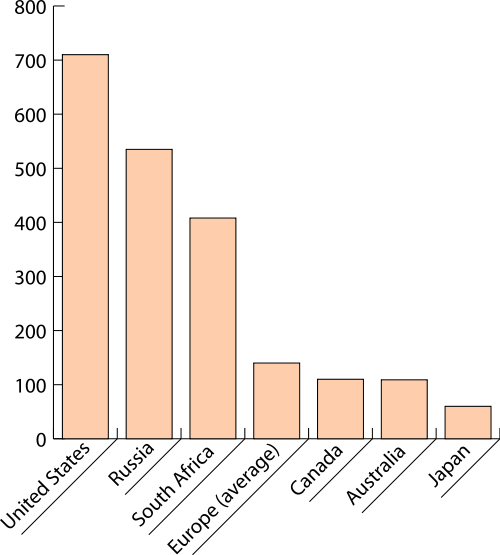
\includegraphics[width=\chartwidth,height=\chartheight]{incarceration}  
\source{Wikipedia}
\end{chart}

\begin{map}{W}{ul}
\caption{Ancient Roma \newline (Trajan times)}
\label{map:roma}
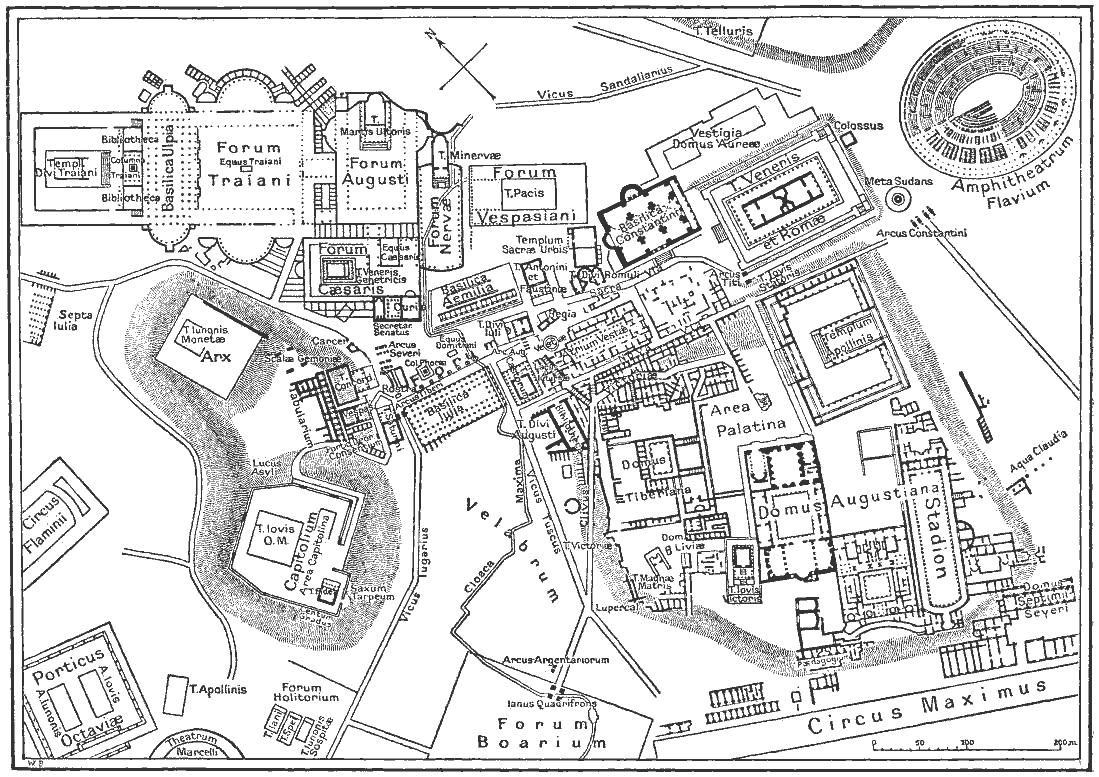
\includegraphics[width=\chartwidth,height=\chartheight]{Rome}
\source{Wikipedia}
\end{map}

\lipsum[1-15]

\begin{chart}{S}{ul}
\caption{Incarceration ratest across countries}
\label{chart:incarceration}
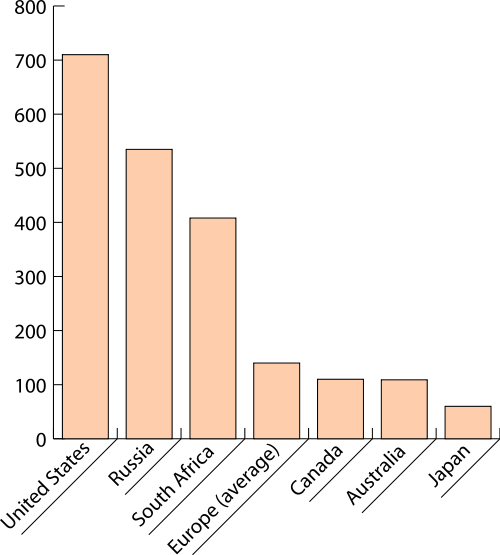
\includegraphics[width=\chartwidth,height=\chartheight]{incarceration}  
\source{Wikipedia}
\end{chart}

\begin{chart}{S}{ll}
\caption{Incarceration ratest acroos countries: First ll chart}
\label{chart:incarceration}
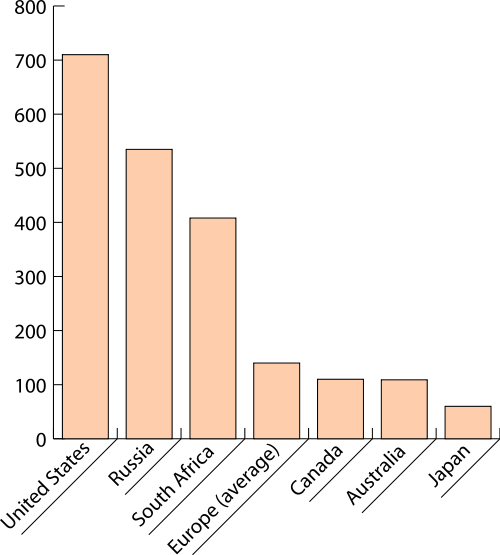
\includegraphics[width=\chartwidth,height=\chartheight]{incarceration}  
\source{Wikipedia}
\end{chart}
\textcolor{red}{a}\footnote{b\\c\\d}
\clearspread

\begin{chart}{S}{ll}
\caption{Incarceration ratest across countries: Second ll chart}
\label{chart:incarceration}
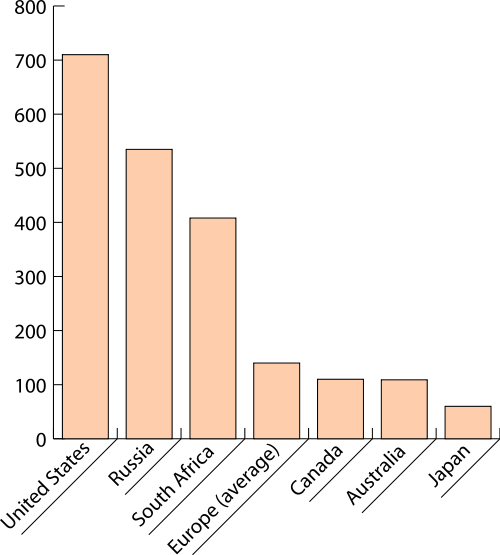
\includegraphics[width=\chartwidth,height=\chartheight]{incarceration}  
\source{Wikipedia}
\end{chart}
\begin{chart}{S}{ll}
\caption{Incarceration ratest across countries: Third ll chart}
\label{chart:incarceration}
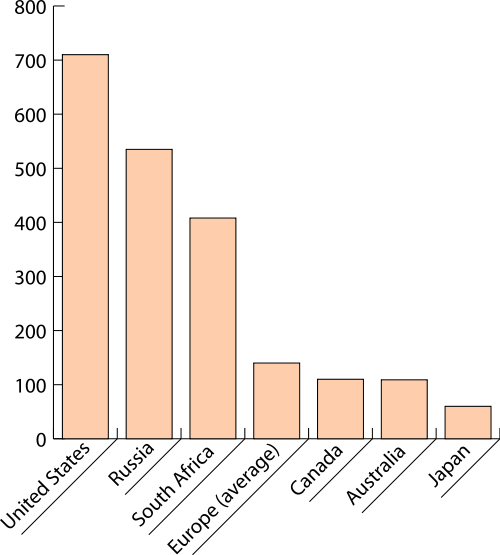
\includegraphics[width=\chartwidth,height=\chartheight]{incarceration}  
\source{Wikipedia}
\end{chart}
\lipsum

\end{document}

